
\begin{frame}
    \frametitle{What even is \LaTeX{}?}
    \framesubtitle<3->{And why should \textit{you} use it?}
    \begin{columns}
    \begin{column}{.47\textwidth}
    \action<2->{It's a typesetting language!}
    \begin{itemize}
        \item Markdown
        \item Word
        \item Adobe Indesign
        \item Affinity Publisher
        \note[item]{%
            In the world of typesetting there are two types of editors:
            Appearance before structure:
                - Adobe Illustrator
                - Affinity Designer
                - Inkscape
            Structure before appearance:
                - Markdown
                - LaTeX
                - Typst
            Stuff inbetween (worse at both): 
                - Word
                - Pages
        }
    \end{itemize}
    \end{column}
    \begin{column}{.52\textwidth}
    \action<3->{%
    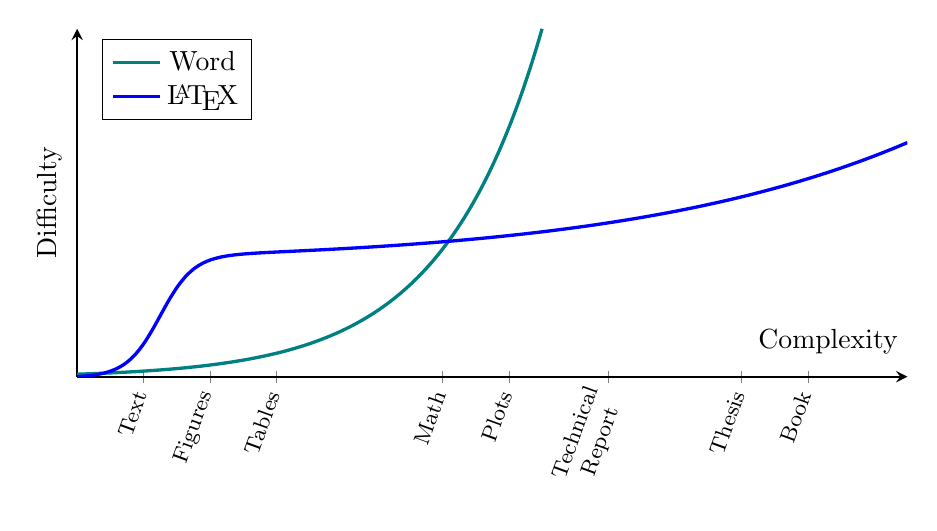
\begin{tikzpicture}
    \begin{axis}[
        smooth, samples = 100,
        axis lines = left,
        axis line style = { thick },
        width = \textwidth,
        height = 6cm,
        grid style = dashed,
        xlabel = Complexity,
        ylabel = Difficulty,
        x label style={at={(axis description cs:1,.1)},anchor=east},
        ytick = \empty,
        xtick = {2, 4, 6, 11, 13, 16, 20, 22},
        xticklabels = {Text, Figures, Tables, Math, Plots, {Technical\\ Report}, Thesis, Book},
        xticklabel style = {align = center},
        x tick label style = { rotate = 70, anchor = east, font=\footnotesize },
        legend style = { legend pos = north west },
        no markers, domain = 0:25,
    ]
        \plot[very thick, teal, domain=0:14]{exp(x/3 - 2.5)};
        \addlegendentry{Word}
        \plot[very thick, blue]{3/(1 + exp(-2*(x-2.5))) + x/50*exp((x-4)/12)};
        \addlegendentry{\textrm{\LaTeX}}
    \end{axis}
    \end{tikzpicture}}
    \end{column}
    \end{columns}
\end{frame}